\documentclass{standalone}
\usepackage{tikz}
\usetikzlibrary{patterns, positioning}
\usepackage[sfdefault]{ClearSans} %% option 'sfdefault' activates Clear Sans as the default text font
\usepackage[T1]{fontenc}

\begin{document}
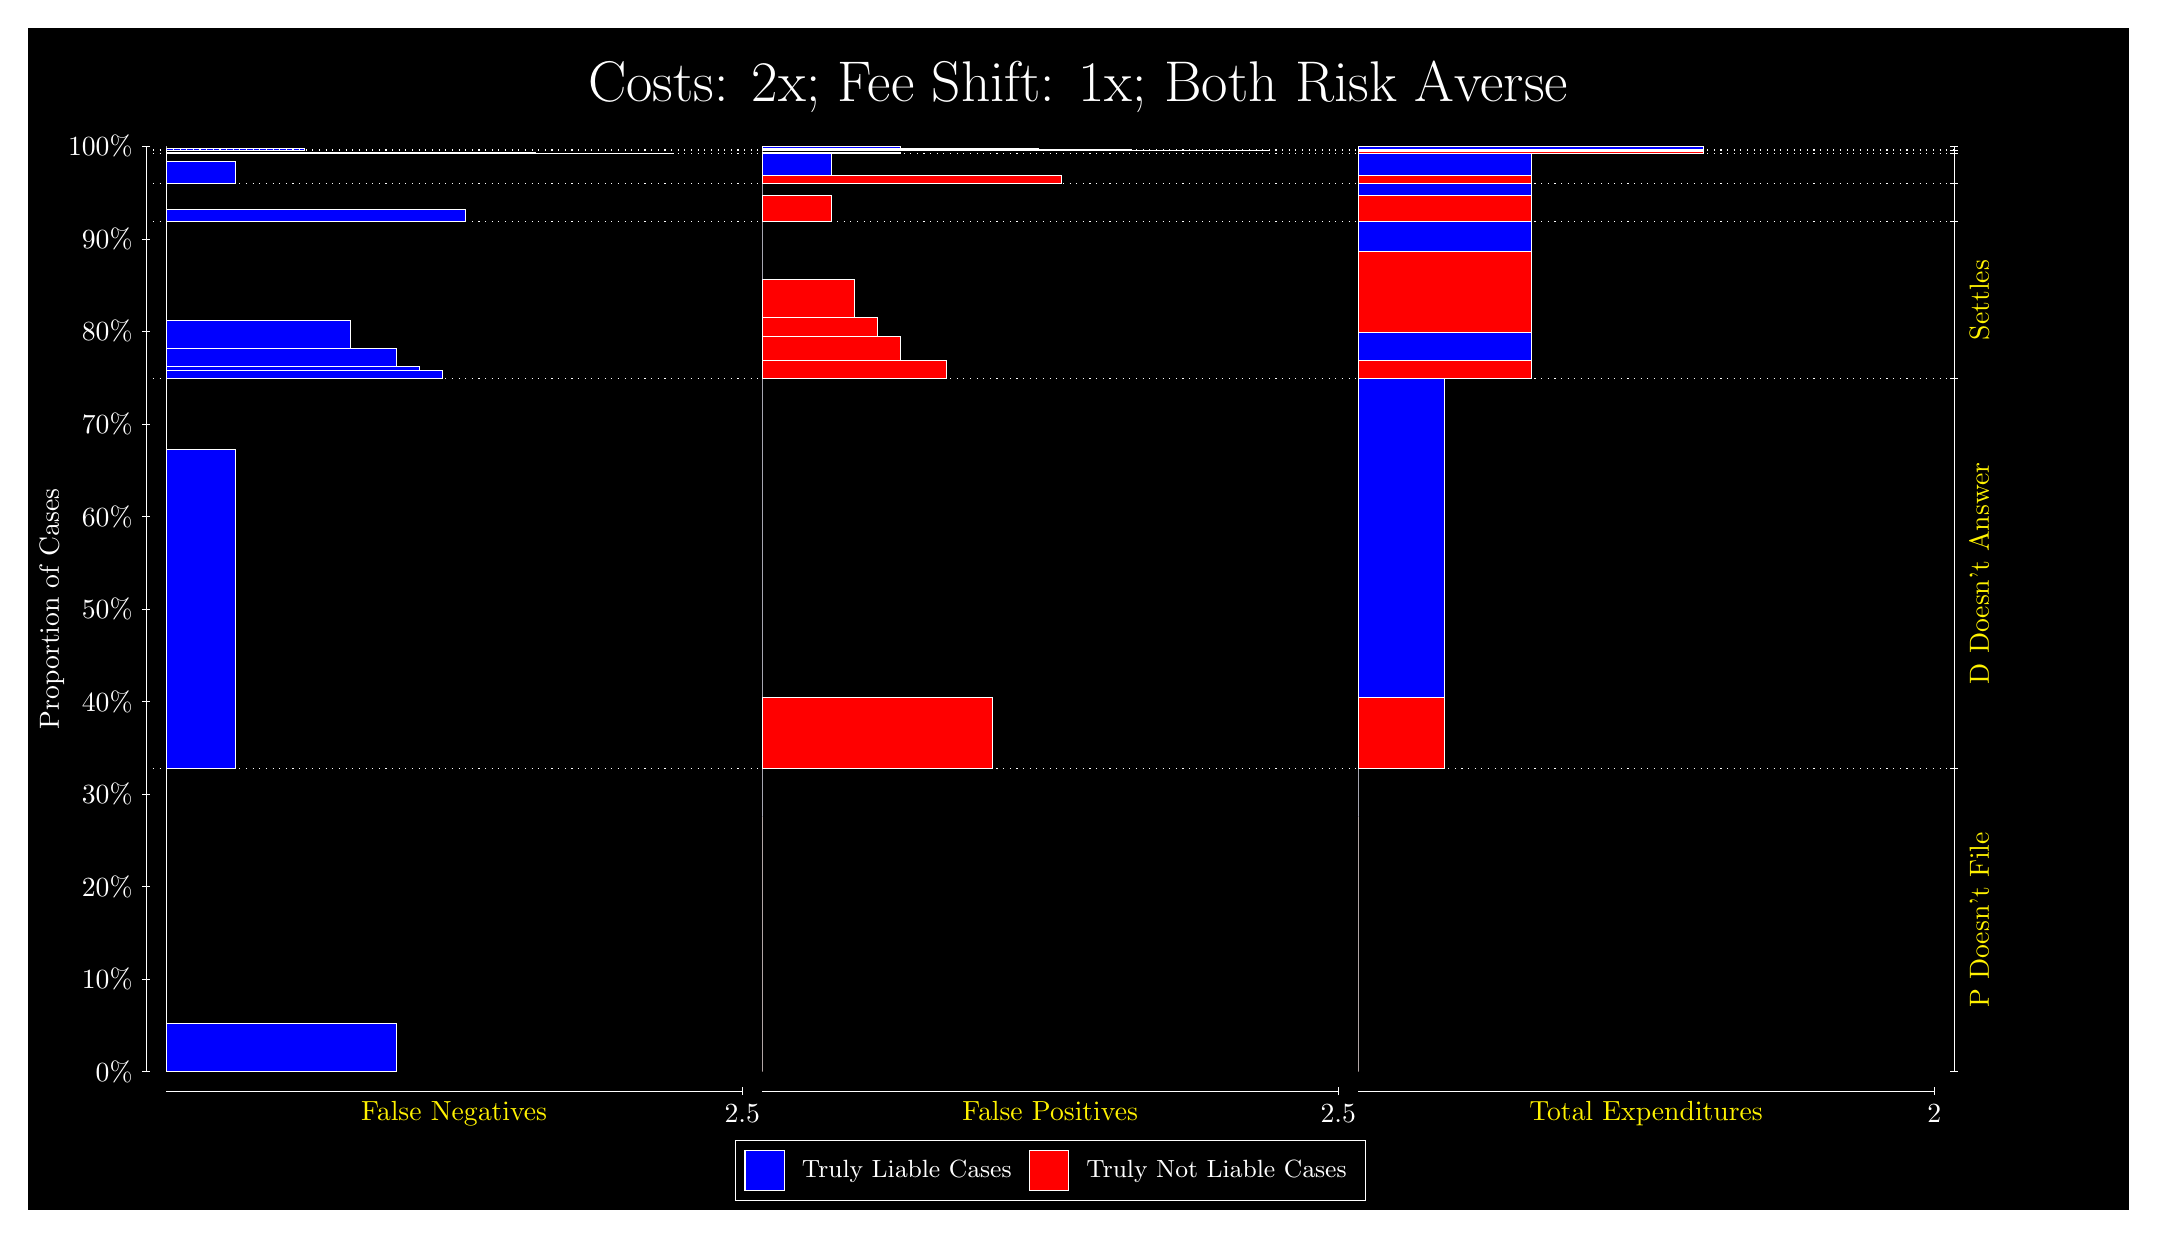
\begin{tikzpicture}
\draw[fill=black] (0,0) rectangle (26.667,15);
\draw[text=white] (0,13.5) rectangle (26.667,15) node[midway] {\huge Costs: 2x; Fee Shift: 1x; Both Risk Averse};
\draw[white, very thin] (1.5,1.75) -- (1.5,13.5);
\node[rotate=90, text=white, anchor=center] at (0.3, 7.625) {Proportion of Cases};
\draw[white, very thin] (1.45,1.75) -- (1.55,1.75);
\node[text=white, anchor=east] at (1.45, 1.75) {0\%};
\draw[white, very thin] (1.45,2.925) -- (1.55,2.925);
\node[text=white, anchor=east] at (1.45, 2.925) {10\%};
\draw[white, very thin] (1.45,4.1) -- (1.55,4.1);
\node[text=white, anchor=east] at (1.45, 4.1) {20\%};
\draw[white, very thin] (1.45,5.275) -- (1.55,5.275);
\node[text=white, anchor=east] at (1.45, 5.275) {30\%};
\draw[white, very thin] (1.45,6.45) -- (1.55,6.45);
\node[text=white, anchor=east] at (1.45, 6.45) {40\%};
\draw[white, very thin] (1.45,7.625) -- (1.55,7.625);
\node[text=white, anchor=east] at (1.45, 7.625) {50\%};
\draw[white, very thin] (1.45,8.8) -- (1.55,8.8);
\node[text=white, anchor=east] at (1.45, 8.8) {60\%};
\draw[white, very thin] (1.45,9.975) -- (1.55,9.975);
\node[text=white, anchor=east] at (1.45, 9.975) {70\%};
\draw[white, very thin] (1.45,11.15) -- (1.55,11.15);
\node[text=white, anchor=east] at (1.45, 11.15) {80\%};
\draw[white, very thin] (1.45,12.325) -- (1.55,12.325);
\node[text=white, anchor=east] at (1.45, 12.325) {90\%};
\draw[white, very thin] (1.45,13.5) -- (1.55,13.5);
\node[text=white, anchor=east] at (1.45, 13.5) {100\%};

\draw[white, very thin] (24.457,1.75) -- (24.457,13.5);
\draw[white, very thin] (24.407,1.75) -- (24.507,1.75);
\node[anchor=west] at (24.407, 1.75) {};
\draw[white, very thin] (24.407,5.6) -- (24.507,5.6);
\node[anchor=west] at (24.407, 5.6) {};
\draw[white, very thin] (24.407,10.551) -- (24.507,10.551);
\node[anchor=west] at (24.407, 10.551) {};
\draw[white, very thin] (24.407,12.547) -- (24.507,12.547);
\node[anchor=west] at (24.407, 12.547) {};
\draw[white, very thin] (24.407,13.032) -- (24.507,13.032);
\node[anchor=west] at (24.407, 13.032) {};
\draw[white, very thin] (24.407,13.412) -- (24.507,13.412);
\node[anchor=west] at (24.407, 13.412) {};
\draw[white, very thin] (24.407,13.453) -- (24.507,13.453);
\node[anchor=west] at (24.407, 13.453) {};
\draw[white, very thin] (24.407,13.5) -- (24.507,13.5);
\node[anchor=west] at (24.407, 13.5) {};

\draw[white, very thin, fill=blue] (1.75,1.75) rectangle (4.6775,2.3639);
\draw[white, very thin, fill=red] (1.75,2.3639) rectangle (1.75,5.6);
\draw[white, very thin, fill=blue] (1.75,5.6) rectangle (2.6283,9.6473);
\draw[white, very thin, fill=red] (1.75,9.6473) rectangle (1.75,10.551);
\draw[white, very thin, fill=blue] (1.75,10.551) rectangle (5.2631,10.656);
\draw[white, very thin, fill=blue] (1.75,10.656) rectangle (4.9703,10.712);
\draw[white, very thin, fill=blue] (1.75,10.712) rectangle (4.6775,10.933);
\draw[white, very thin, fill=blue] (1.75,10.933) rectangle (4.092,11.29);
\draw[white, very thin, fill=red] (1.75,11.29) rectangle (1.75,12.547);
\draw[white, very thin, fill=blue] (1.75,12.547) rectangle (5.5558,12.696);
\draw[white, very thin, fill=red] (1.75,12.696) rectangle (1.75,13.032);
\draw[white, very thin, fill=blue] (1.75,13.032) rectangle (2.6283,13.31);
\draw[white, very thin, fill=red] (1.75,13.31) rectangle (1.75,13.412);
\draw[white, very thin, fill=blue] (1.75,13.412) rectangle (8.1906,13.415);
\draw[white, very thin, fill=blue] (1.75,13.415) rectangle (6.4341,13.426);
\draw[white, very thin, fill=red] (1.75,13.426) rectangle (1.75,13.453);
\draw[white, very thin, fill=blue] (1.75,13.453) rectangle (3.5065,13.471);
\draw[white, very thin, fill=red] (1.75,13.471) rectangle (1.75,13.486);
\draw[white, very thin, fill=blue] (1.75,13.486) rectangle (1.75,13.5);
\draw[white, very thin, fill=red] (9.3189,1.75) rectangle (9.3189,4.9861);
\draw[white, very thin, fill=blue] (9.3189,4.9861) rectangle (9.3189,5.6);
\draw[white, very thin, fill=red] (9.3189,5.6) rectangle (12.246,6.504);
\draw[white, very thin, fill=blue] (9.3189,6.504) rectangle (9.3189,10.551);
\draw[white, very thin, fill=red] (9.3189,10.551) rectangle (11.661,10.782);
\draw[white, very thin, fill=red] (9.3189,10.782) rectangle (11.075,11.091);
\draw[white, very thin, fill=red] (9.3189,11.091) rectangle (10.783,11.335);
\draw[white, very thin, fill=red] (9.3189,11.335) rectangle (10.49,11.808);
\draw[white, very thin, fill=blue] (9.3189,11.808) rectangle (9.3189,12.547);
\draw[white, very thin, fill=red] (9.3189,12.547) rectangle (10.197,12.883);
\draw[white, very thin, fill=blue] (9.3189,12.883) rectangle (9.3189,13.032);
\draw[white, very thin, fill=red] (9.3189,13.032) rectangle (13.125,13.134);
\draw[white, very thin, fill=blue] (9.3189,13.134) rectangle (10.197,13.412);
\draw[white, very thin, fill=red] (9.3189,13.412) rectangle (11.075,13.428);
\draw[white, very thin, fill=red] (9.3189,13.428) rectangle (9.3189,13.438);
\draw[white, very thin, fill=blue] (9.3189,13.438) rectangle (9.3189,13.453);
\draw[white, very thin, fill=red] (9.3189,13.453) rectangle (15.759,13.456);
\draw[white, very thin, fill=red] (9.3189,13.456) rectangle (14.003,13.467);
\draw[white, very thin, fill=blue] (9.3189,13.467) rectangle (12.832,13.481);
\draw[white, very thin, fill=blue] (9.3189,13.481) rectangle (11.075,13.5);
\draw[white, very thin, fill=red] (16.888,1.75) rectangle (16.888,4.9861);
\draw[white, very thin, fill=blue] (16.888,4.9861) rectangle (16.888,5.6);
\draw[white, very thin, fill=red] (16.888,5.6) rectangle (17.986,6.504);
\draw[white, very thin, fill=blue] (16.888,6.504) rectangle (17.986,10.551);
\draw[white, very thin, fill=red] (16.888,10.551) rectangle (19.083,10.782);
\draw[white, very thin, fill=blue] (16.888,10.782) rectangle (19.083,11.138);
\draw[white, very thin, fill=red] (16.888,11.138) rectangle (19.083,12.164);
\draw[white, very thin, fill=blue] (16.888,12.164) rectangle (19.083,12.547);
\draw[white, very thin, fill=red] (16.888,12.547) rectangle (19.083,12.883);
\draw[white, very thin, fill=blue] (16.888,12.883) rectangle (19.083,13.032);
\draw[white, very thin, fill=red] (16.888,13.032) rectangle (19.083,13.134);
\draw[white, very thin, fill=blue] (16.888,13.134) rectangle (19.083,13.412);
\draw[white, very thin, fill=red] (16.888,13.412) rectangle (21.279,13.438);
\draw[white, very thin, fill=blue] (16.888,13.438) rectangle (21.279,13.453);
\draw[white, very thin, fill=red] (16.888,13.453) rectangle (21.279,13.467);
\draw[white, very thin, fill=blue] (16.888,13.467) rectangle (21.279,13.5);
\draw[white, dotted] (1.5,5.6) -- (24.457,5.6);
\draw[white, dotted] (1.5,10.551) -- (24.457,10.551);
\draw[white, dotted] (1.5,12.547) -- (24.457,12.547);
\draw[white, dotted] (1.5,13.032) -- (24.457,13.032);
\draw[white, dotted] (1.5,13.412) -- (24.457,13.412);
\draw[white, dotted] (1.5,13.453) -- (24.457,13.453);
\draw[white, very thin] (1.75,1.5) -- (9.0689,1.5);
\node[text=yellow, anchor=north] at (5.4094, 1.5) {False Negatives};
\draw[white, very thin] (9.0689,1.45) -- (9.0689,1.55);
\node[text=white, anchor=north] at (9.0689, 1.45) {2.5};

\draw[white, very thin] (9.3189,1.5) -- (16.638,1.5);
\node[text=yellow, anchor=north] at (12.978, 1.5) {False Positives};
\draw[white, very thin] (16.638,1.45) -- (16.638,1.55);
\node[text=white, anchor=north] at (16.638, 1.45) {2.5};

\draw[white, very thin] (16.888,1.5) -- (24.207,1.5);
\node[text=yellow, anchor=north] at (20.547, 1.5) {Total Expenditures};
\draw[white, very thin] (24.207,1.45) -- (24.207,1.55);
\node[text=white, anchor=north] at (24.207, 1.45) {2};

\node[text=yellow, centered, rotate=90] at (24.777, 3.675) {P Doesn't File};
\node[text=yellow, centered, rotate=90] at (24.777, 8.0756) {D Doesn't Answer};
\node[text=yellow, centered, rotate=90] at (24.777, 11.549) {Settles};





\draw (12.978300999999998,1.5) node[draw=none] (baseCoordinate) {};
\begin{scope}[align=center]
        \matrix[scale=0.5, draw=white, below=0.5cm of baseCoordinate, nodes={draw}, column sep=0.1cm]{
            \node[rectangle, draw, minimum width=0.5cm, minimum height=0.5cm, fill=blue] {}; &
            \node[draw=none, font=\small, text=white] (B) {Truly Liable Cases}; &
            \node[rectangle, draw, minimum width=0.5cm, minimum height=0.5cm, fill=red] {}; &
            \node[draw=none, font=\small, text=white] (B) {Truly Not Liable Cases}; \\
            };
\end{scope}

\end{tikzpicture}
\end{document}